\documentclass[10pt,twocolumn,letterpaper]{article}

\usepackage{iccv}
\usepackage{times}
\usepackage{epsfig}
\usepackage{graphicx}
\usepackage{amsmath}
\usepackage{amssymb}
\usepackage{algorithm}
\usepackage{algpseudocode}

\usepackage[breaklinks=true,bookmarks=false]{hyperref}

\iccvfinalcopy % *** Uncomment this line for the final submission

\begin{document}

%%%%%%%%% TITLE
\title{Dynamic Viewing\\CS280 Final Project}

\author{Rohan Chitnis\\
23464697\\
{\tt\small ronuchit@berkeley.edu}
\and
Alan Yao\\
23775635\\
{\tt\small alanyao@berkeley.edu}
\and
Alexander Chu\\
23460953\\
{\tt\small alex.p.chu@berkeley.edu}
}

\maketitle

\begin{abstract}
  Fast online tracking algorithms are fundamental to many real-world computer
  vision applications, such as video segmentation and human-computer interaction.
  We develop a multiscale sum-of-squared-displacements (SSD) template matching algorithm for
  tracking an object in a live video feed. Furthermore, we build invariance
  to rotation and scale directly into our system using linear interpolation on heuristic
  score functions. We evaluate performance through comparison with OpenCV's tracking
  algorithms based on Haar cascades \cite{haarcascade} and show that our system performs comparably to or
  better than OpenCV in all accuracy metrics, with a considerable improvement to
  lighting and background invariance.
\end{abstract}

\section*{Introduction}
3d graphics on monitors are unrealistic because they assume a center of projection
some distance away from the center of the screen. That is, they assume the viewer
is at a certain fixed position (usually in front of the middle of the screen) when
generating the projection. If the position of the viewer is known, however, the
center of projection can be set to match the viewer's point of view. As an analogy,
looking at the monitor will thus be much akin to looking through a window: the observed
scene undergoes certain projective transformations based on where the viewer is standing
relative to the window.\\

We develop an algorithm to track the position of an object
during a live webcam video feed. In order to achieve online tracking, which necessitates
quick computations, we use multiscale SSD template matching to determine the location of
the object. Additionally, we incorporate rotation and scale invariance, which allows us to
compute orientation and distance, and update the scene accordingly. We validate our
approach in a simulated computer game environment and through experimental comparisons
with OpenCV's implementation of facial tracking using Haar cascades.

\section*{Approach}

\subsection*{Multiscale SSD for Tracking}
SSD$(I, J)$ of two images $I$ and $J$ is computed as
$$\displaystyle\sum_{i, j}(I_{ij} - J_{ij})^{2}$$

At the heart of our system is a multiscale SSD template matcher, which operates as follows.
Initially, the user is asked to place his or her face inside an axis-aligned square window of size
$m$ by $m$. The image inside this window is then used as a template for the online
portion of the tracking. A naive SSD-based approach would then proceed by sliding a window of
size $m$ by $m$ across the online image captured by the webcam, performing SSD at each window,
and returning the window position corresponding to the minimum SSD. However, our initial
experimentation found this approach to be much too slow (enabling us to only reach about 10 FPS
in an online setting, which would have deproved upon introducing rotation and scale invariance).\\

In order to remedy this, we instead operate on multiple scales of both the online image and the
template image, by constructing a Gaussian pyramid \cite{gpyr} and running the full sliding window for only
the topmost level of the pyramid. Then, once we have found the optimal window position which
minimizes SSD here, we have a small range within which we may search the next lowest level of
the pyramid. This continues until we have found the optimal window position for our original image.
This algorithm requires keeping track of the SSD search range at the current pyramid level.
Pseudocode for our implementation is described in Algorithm 1.\\

\begin{algorithm}
 \caption{Multiscale SSD sliding window for tracking.}
 \begin{algorithmic}[1]
  \Procedure{DetermineBestShift}{ImagePyramid, TemplatePyramid}
  \State $m \leftarrow$ window side length
  \State $N \leftarrow$ pyramid size
  \State wa $\leftarrow \lfloor m / 2^{N} \rfloor$
  \State tip $\leftarrow$ Topmost(ImagePyramid)
  \State ttp $\leftarrow$ Topmost(TemplatePyramid)
  \State r\_inds $\leftarrow$ (0, (tip.height - ttp.height) / wa,\\\hspace{57pt}0, (tip.width - ttp.width) / wa)
  \For {$i$ = $N$ \textbf{downto} 1}
     \State cip $\leftarrow$ ImagePyramid[$i$]
     \State ctp $\leftarrow$ TemplatePyramid[$i$]
     \State best\_i, best\_j $\leftarrow$ DoSSD(cip, ctp, $2^{i}$, r\_inds)
     \State r\_inds $\leftarrow$ (best\_i - 1, best\_i + 1,\\\hspace{73pt}best\_j - 1, best\_j + 1)
  \EndFor
  \State \Return best\_i, best\_j
  \EndProcedure
 \end{algorithmic}
  \begin{algorithmic}[1]
  \Procedure{DoSSD}{Image, Template, scaleAmt, r\_inds}
  \State $m \leftarrow$ window side length
  \State wa $\leftarrow \lfloor m / \text{scaleAmt} \rfloor$
  \State w $\leftarrow$ Template.width
  \State h $\leftarrow$ Template.height
  \For {$i$ = r\_inds[0] \textbf{to} r\_inds[1]}
    \For {$j$ = r\_inds[2] \textbf{to} r\_inds[3]}
    \State cand\_roi $\leftarrow$ Image[wa*i:wa*i+h,\\\hspace{122pt}wa*j:wa*j+w]
    \State calculate SSD(Template, cand\_roi)
    \EndFor
  \EndFor
  \State \Return $i$, $j$ having minimum SSD
  \EndProcedure
 \end{algorithmic}
\end{algorithm}

Some clarifications of Algorithm 1 are in order. The variable \texttt{wa}
represents the window size at the current pyramid level. The variable \texttt{r\_inds}
is a tuple of the form (start $i$, end $i$, start $j$, end $j$); it keeps
track of the region of the online image within which the SSD must be computed
at this level of the pyramid, in units of window size (this is why it gets
multiplied by \texttt{wa} in the calculation of the candidate region, at line 8 of
DoSSD). Note that the algorithm assumes a downsampling factor of 2 at each level
of the two pyramids.

\subsection*{Building Invariance}
Algorithm 1, multiscale SSD, only provides translational invariance between the
template image and the online image. However, this is limited in utility, so we
extend the algorithm to provide rotational and scale invariance, and in the
process we develop a method of determining the orientation and scale both quickly
and accurately. If one had infinite computational resources, one would discretize
each of these quantities into a large number of buckets and run Algorithm 1 for
the template at each quantity. For example, one could imagine running Algorithm 1 on the template
image rotated each degree from -45 to 45, and take the orientation which minimizes SSD.
However, this is clearly not computationally feasible.\\

Instead, we propose the following approach. For orientation, we run Algorithm 1
on the template image rotated to a small number of preset orientations, then based on the SSD value
of each of these, we perform linear interpolation to estimate the current orientation.
The interpolation weights are based on the SSD values: since a lower SSD means we want
to give this rotation amount a higher weight, we use the multiplicative inverse of the
SSD for the interpolation weights. The general formula then becomes
$$rot = \displaystyle\sum_{k}(\dfrac{1.0 / SSD_{k}}{\sum_{k'}(1.0 / SSD_{k'})} * rots[k])$$
where $rots$ is an array that holds all the preset rotation amounts in degrees,
the summation is over the indices of this array, and $SSD_{k}$ represents the SSD value
corresponding to the rotation amount $rots[k]$.

Similarly,
$$scale = \displaystyle\sum_{k}(\dfrac{1.0 / SSD_{k}}{\sum_{k'}(1.0 / SSD_{k'})} * scale[k])$$

Note that this requires storage of online pyramids and template pyramids corresponding
to each of the preset rotation amounts and scale amounts.

\subsection*{Rendering Engine Updates}
We ask the user to start with his or her face approximately 1 foot away from the screen. This allows us to estimate the focal length $f$ of the camera, using
$$f = width_{face} * \frac{start\ distance}{average\ face\ width}$$
This also allows us to get $(x_c, y_c)$, the starting center point of the user's face off which we base translations.
Then, for any online image (frame capture), we use the algorithms previously described to obtain $x_i, x_j, rot_{interp}, scale_{interp}$, where $rot_{interp}$ refers to the rotation amount of the face around the center of the face, and $scale_{interp}$ refers to the width of the scaled bounding box, which we always consider to be a square. From these parameters we can calculate the updated camera transforms as:
$$Z = f - f \frac{scale_{interp}}{width_{window}}$$
$$x_{rot}, y_{rot} = tan^{-1}(\frac{(x_i,y_i)-(x_c,y_c)}{Z})$$
We then rotate around the $x$ and $y$ axes by $x_{rot}, y_{rot}$ and around the viewing axis by $rot_{interp}$. We translate the camera along the viewing axis by $Z$.

\subsection*{Real Time Smoothing}
Because SSD still only gives us face position tracking data at a finite framerate, we perform real time smoothing and interpoltation using a Kalman filter. We represent the state of the face (position, velocity, and acceleration) as a vector, and apply a linear dynamics model to predict the next position of the face. We then weight the prediction against any new face tracking data that may be available at a given time. Our specific implementation of the Kalman filter is based on Meinhold and Singpurwalla's work \cite{kalman}.

We experimented with two different dynamics models for real time smoothing. First, we modeled the position, velocity, and acceleration as part of the state space. We then tried modeling only position and velocity, assuming zero local acceleration. The resulting dynamics updates are shown below:

\textbf{Position, Velocity, and Acceleration}
$$ x_t =\begin{bmatrix}
  1 & T & 0 & 0 & 0 & 0 & 0 & 0 & 0 \\
  0 & 1 & T & 0 & 0 & 0 & 0 & 0 & 0 \\
  0 & 0 & 1 & 0 & 0 & 0 & 0 & 0 & 0 \\
  0 & 0 & 0 & 1 & T & 0 & 0 & 0 & 0 \\
  0 & 0 & 0 & 0 & 1 & T & 0 & 0 & 0 \\
  0 & 0 & 0 & 0 & 0 & 1 & 0 & 0 & 0 \\
  0 & 0 & 0 & 0 & 0 & 0 & 1 & T & 0 \\
  0 & 0 & 0 & 0 & 0 & 0 & 0 & 1 & T \\
  0 & 0 & 0 & 0 & 0 & 0 & 0 & 0 & 1 \\
\end{bmatrix} x_{t-1},
x =
\begin{bmatrix}
  x \\
  v_{x} \\
  a_{x} \\
  y \\
  v_{y} \\
  a_{y} \\
  z \\
  v_{z} \\
  a_{zt} \\
\end{bmatrix}$$

\textbf{Position and Velocity}
$$ x_t =\begin{bmatrix}
  1 & T & 0 & 0 & 0 & 0 \\
  0 & 1 & 0 & 0 & 0 & 0 \\
  0 & 0 & 1 & T & 0 & 0 \\
  0 & 0 & 0 & 1 & 0 & 0 \\
  0 & 0 & 0 & 0 & 1 & T \\
  0 & 0 & 0 & 0 & 0 & 1 \\
\end{bmatrix} x_{t-1},
x =
\begin{bmatrix}
  x \\
  v_{x} \\
  y \\
  v_{y} \\
  z \\
  v_{z} \\
\end{bmatrix}$$

Including acceleration in the model allows us to fully model the entire range of kinematic motion. However, it also made the model much more sensitive to noise from the face tracker. Modeling the dynamics using locally constant velocity, on the other hand, produced smooth, real time interpolations between face tracking frames. 

\subsection*{Eliminating False Positives}

\begin{figure}[ht!]
\centering
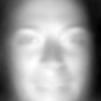
\includegraphics[width=20mm]{./eigenface/eigenfaces/1.jpg}
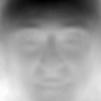
\includegraphics[width=20mm]{./eigenface/eigenfaces/2.jpg}
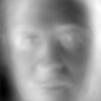
\includegraphics[width=20mm]{./eigenface/eigenfaces/3.jpg}
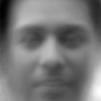
\includegraphics[width=20mm]{./eigenface/eigenfaces/4.jpg}
\caption{Some Eigenfaces.\label{overflow}}
\end{figure}

\begin{figure}[ht!]
\centering
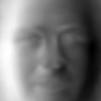
\includegraphics[width=20mm]{./eigenface/reconstruction/face_proj_1.jpg}
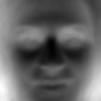
\includegraphics[width=20mm]{./eigenface/reconstruction/face_proj_10.jpg}
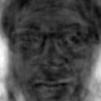
\includegraphics[width=20mm]{./eigenface/reconstruction/face_proj_100.jpg}
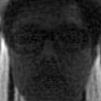
\includegraphics[width=20mm]{./eigenface/reconstruction/face_proj_1000.jpg}
\caption{Reconstruction of a face: 1, 10, 100, 1000 eigenfaces.\label{overflow}}
\end{figure}

\begin{figure}[ht!]
\centering
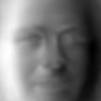
\includegraphics[width=20mm]{./eigenface/reconstruction/nonface_proj_1.jpg}
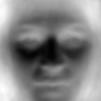
\includegraphics[width=20mm]{./eigenface/reconstruction/nonface_proj_10.jpg}
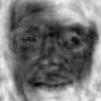
\includegraphics[width=20mm]{./eigenface/reconstruction/nonface_proj_100.jpg}
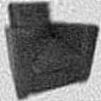
\includegraphics[width=20mm]{./eigenface/reconstruction/nonface_proj_1000.jpg}
\caption{Reconstruction of a chair: 1, 10, 100, 1000 eigenfaces.\label{overflow}}
\end{figure}



One issue we noted is that the SSD algorithm is not good at detecting whether the template image is in the online image or not -- it is only good at tracking the face. We need an algorithm that detects whether the bounding box from the SSD detection actually contains a face or not. For this purpose, we use an Eigenface algorithm \cite{eigenfaces} to determine if the image in the box falls within the space of faces. We first compute 100 eigenfaces from 2000 faces sampled at random from the Labeled Faces in the Wild \cite{lfw} dataset. We then use the following algorithm to determine if a given image is a face:

\begin{algorithm}
 \caption{Face Detection using Eigenface}
 \begin{algorithmic}[1]
  \Procedure{IsFace}{face, eigenfaces, averageFace, threshold}
  \State Resize face to the size of all the eigenfaces.
  \State face $\leftarrow$ (toGreyScale(face) - averageFace)
  \State face $\leftarrow$ face / $||\mbox{face}||$
  \State projection $\leftarrow$ zeros(height(face),width(face))
  \For {eigenface in eigenfaces}
     \State projection += face $\cdot$ eigenface
  \EndFor
  \State face /= max(face)
  \State projection /= max(projection)
  \State \Return $||\mbox{face - projection}||$ < threshold
  \EndProcedure
 \end{algorithmic}
\end{algorithm}

If the object is actually a face, we should get a low reconstruction error, since the object falls within the subspace used in computing the PCA basis for faces. If the object is not a face, we should get a higher reconstruction error. Care must be taken to restrict the dimensionality of the PCA basis used. As seen in figure 2 and 3, reconstruction quality of faces and non-faces differs the most with around 100 eigenfaces for our image size.

\section*{Experiments}

\subsection*{Setting}
We evaluate performance in a simulated computer game environment loosely based
on Minecraft \cite{minecraft}. We feed our webcam image through Algorithm 1 for each rotation
value and each scale value to determine the orientation and distance amounts as well as
the window position which minimizes SSD for these amounts. Then, we use this
information to update the rendering engine as previously described. In our experimentation,
we used rotation amounts of -45, 0, and 45 degrees, and scale amounts of 0.5, 1, and 1.5,
for the interpolation. Furthermore, we used a pyramid size of 3 (where the bottom
layer is simply the original image) and a downsampling factor of 2. Our window amount
was 8, and we assumed the average face size to be 250 pixels.

Our development environment was Python 2.7, and our rendering engine was Pyglet.
\begin{figure}[ht!]
\centering
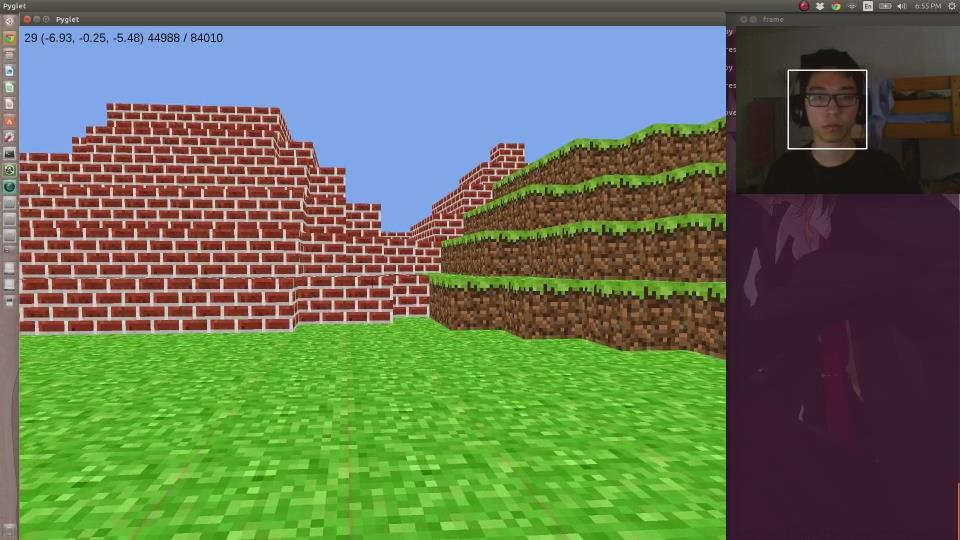
\includegraphics[width=90mm]{left_trans.jpg}
\caption{Initial configuration of head.\label{overflow}}
\end{figure}

\begin{figure}[ht!]
\centering
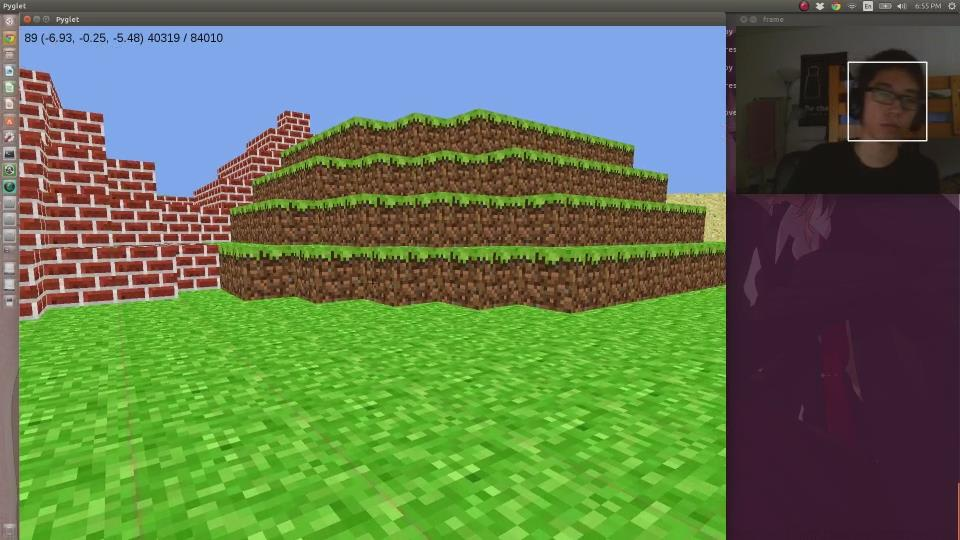
\includegraphics[width=90mm]{right_trans.jpg}
\caption{Moving head to the left.\label{overflow}}
\end{figure}

\begin{figure}[ht!]
\centering
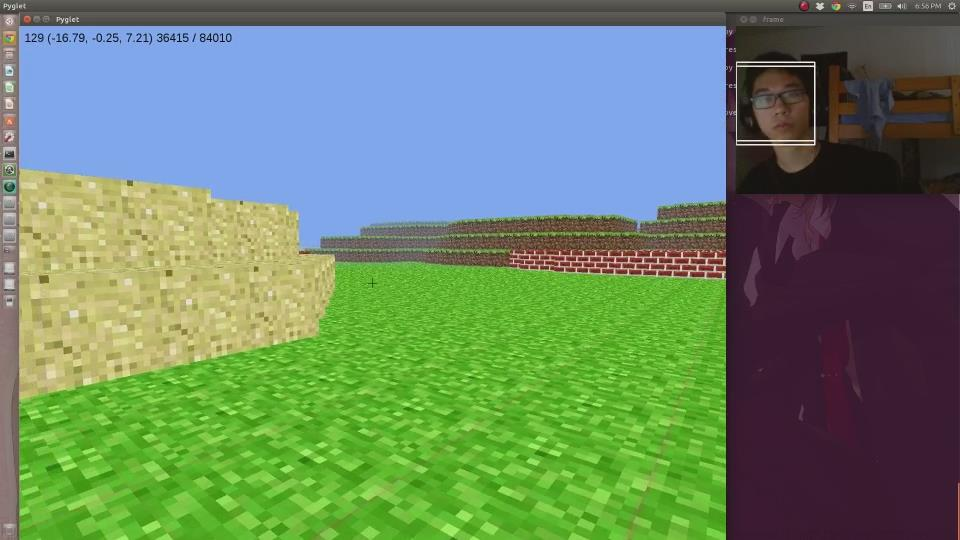
\includegraphics[width=90mm]{forward.jpg}
\caption{Moving head forward and to the right.\label{overflow}}
\end{figure}

\begin{figure}[ht!]
\centering
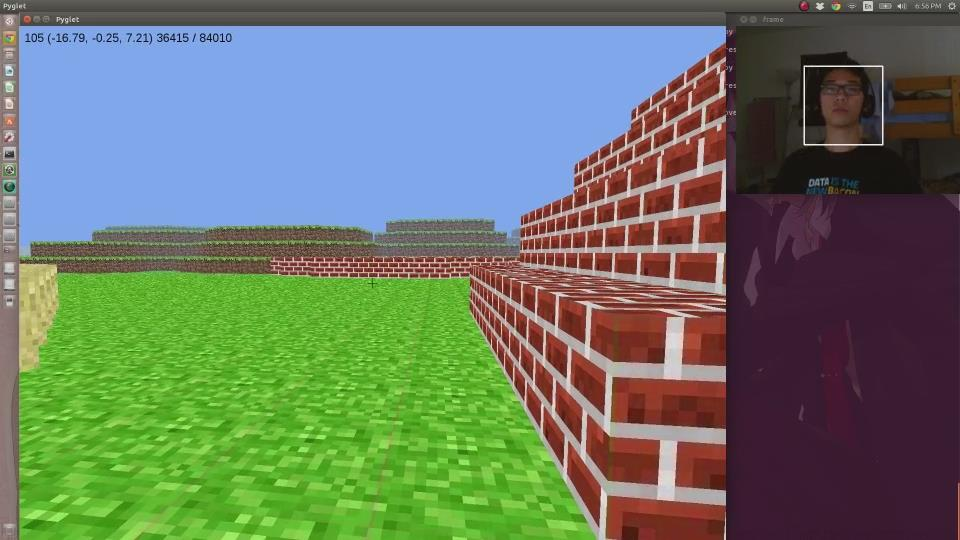
\includegraphics[width=90mm]{back_away.jpg}
\caption{Moving head back.\label{overflow}}
\end{figure}

\begin{figure}[ht!]
\centering
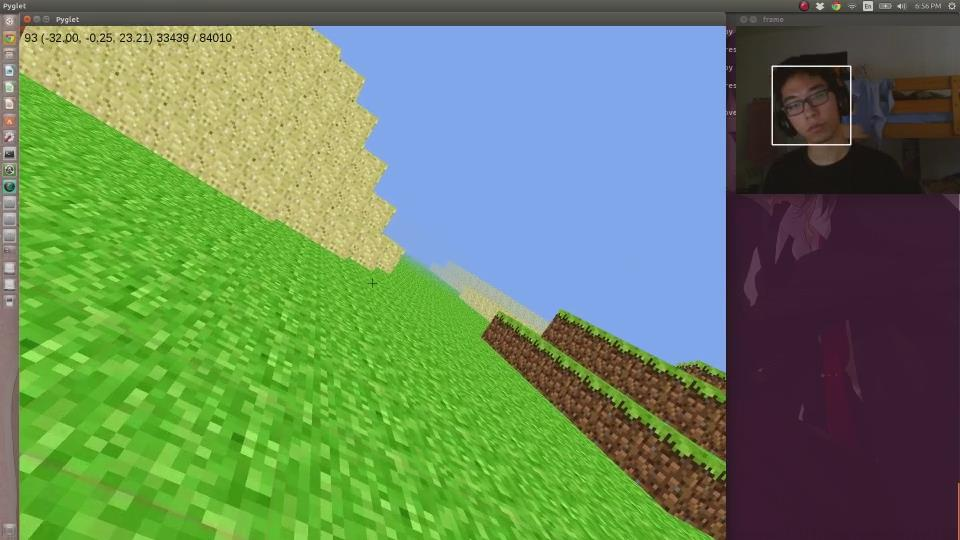
\includegraphics[width=90mm]{rotation_left.jpg}
\caption{Rotating head right.\label{overflow}}
\end{figure}

\begin{figure}[ht!]
\centering
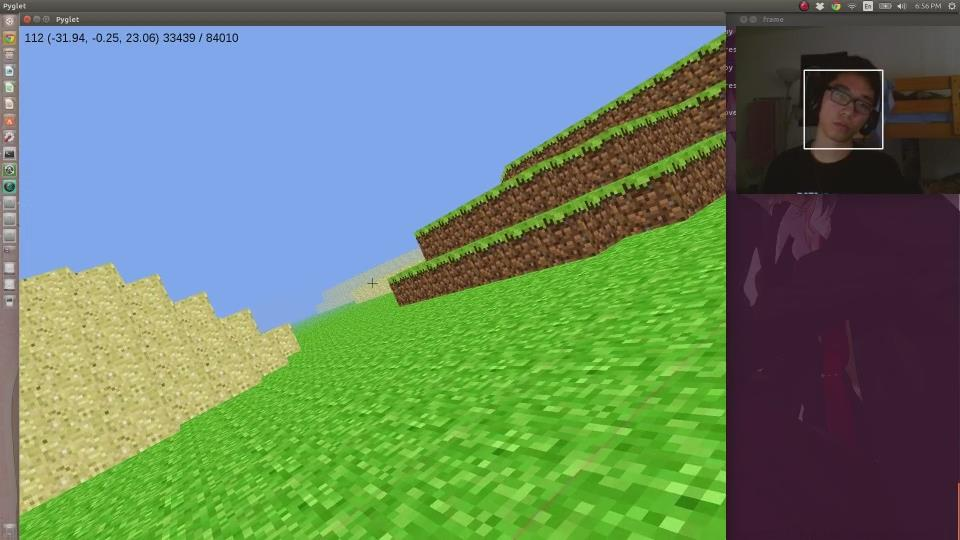
\includegraphics[width=90mm]{rotation_right.jpg}
\caption{Rotating head left.\label{overflow}}
\end{figure}

\subsection*{Results}
We achieve acceptable error rates for scale distance and exact rotation of the face as shown in Figures 1 through 6. In practice, due to smoothing and user perception, the error between exact facial rotation/scale and the computed rotation/scale is not noticeable. Additionally, the algorithm always detects the bounding box of the face correctly. This ensures that the core functionality is not affected.

\begin{figure}[ht!]
\centering
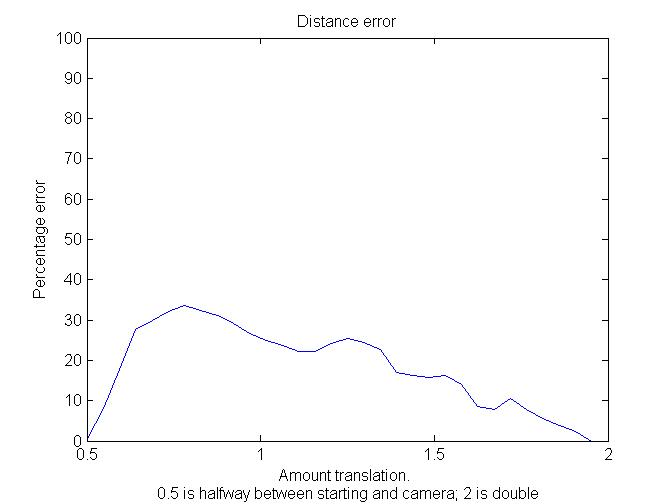
\includegraphics[width=90mm]{distance_error.jpg}
\caption{Scale (distance) error rates.\label{overflow}}
\end{figure}
\begin{figure}[ht!]
\centering
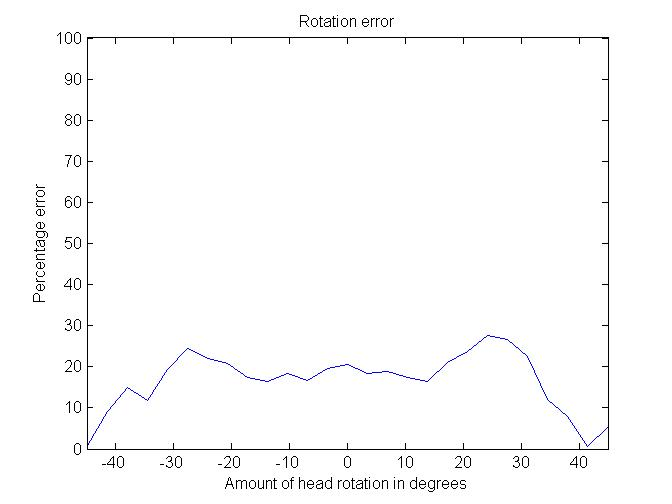
\includegraphics[width=90mm]{rotation_error.jpg}
\caption{Rotation error rates.\label{overflow}}
\end{figure}

\subsection*{Evaluation}
The OpenCV facial Haar cascade classifier achieves similar performance to a naive, single-threaded implementation of our multiscale SSD matcher along with the rotation and scale Gaussian pyramids.
\begin{center}
    \begin{tabular}{| l | l | l |}
    \hline
    \         & \textbf{SSD} & \textbf{OpenCV Haar cascade} \\ \hline
    Face detections per second & 6.28 & 6.15 \\  \hline
    \end{tabular}
\end{center}

However, we achieve noticably higher accuracy on rotated faces, while maintaining the same accuracy on scaled and translated faces. The SSD method is also invariant to backgrounds; the OpenCV Haar cascader doesn't work against a light-colored background or one with strong lighting.

\begin{center}
    \begin{tabular}{| l | l | l |}
    \hline
    \textbf{Setting}                     & \textbf{OpenCV Acc.} & \textbf{SSD Acc.}          \\ \hline
     With background light                  & 0\%       & 100\%       \\ \hline 
     Rotating -45 to 45 degrees           &  20.2\%  & 98.8\%      \\ \hline                 
     Scaling .5 to 2 from original scale & 100\%    & 99.6\%                 \\  \hline
\end{tabular}
\end{center}

After integration into the rendering engine, we can measure the performance of the various methods using the frames per second metric.

\begin{center}
    \begin{tabular}{| l | l |}
    \hline
     \textbf{Method}                                                 & \textbf{FPS}       \\ \hline
     Translation only                                    & 35           \\ \hline 
     Translation + scaling                             &  29           \\ \hline      
    Translation + rotation                            & 28             \\ \hline           
    Translation + scaling + rotation              & 23             \\  \hline
    All, Kalman Filter, background process    & 80             \\   \hline
\end{tabular}
\end{center}

As seen above, by using a Kalman filter to smooth movements, polling less frequently, and farming out the detection process to a background thread, we achieve up to 80 FPS. In fact, the game runs only negligibly faster without the facial tracking at all.

\section*{Conclusion}
The need for fast tracking in an online setting is well-understood and has utility
in several applications of computer vision. We developed and evaluated performance
of an algorithm which uses multiscale SSD template matching and offers invariance to
capture orientation and distance information. We further demonstrated the applicability of our
algorithm by illustrating real-time performance in a simulated computer game environment,
and compared its performance to that of OpenCV. Our code is fully open-source and available
at \url{https://github.com/alancyao/dynamic-viewing}.

{\small
\bibliographystyle{ieee}
\bibliography{egbib}
}

\end{document}
